\oz{} can be used to model an entity with unchanged behavior, but sometimes we need to model an entity that changes its behavior. We introduce dynamic \oz{}, which is a version of \oz{} that uses the state pattern to model an entity with varying behavior.
\subsubsection{OZ and state pattern}
The state pattern is a behavioral software design pattern. An object changes its class when its internal state changes. To illustrate the idea imagine that our vending machine \textit{VM} is a mobile vending machine and that it is connected by a wireless link $talk$ to a shop \textit{Shop1}. On signal fading \textit{Shop1} decides to send the link \textit{talk} to another shop \textit{Shop2} through the link \textit{switch} as shown in \refFig{fig_oz_mobile_vending_machine_and_shops}. \textit{Shop1, Shop2} change their behavior after switching. This varying behavior of shop can be handled through by using two classes \textit{ActiveShop, IdleShop} . A shop changes its class when \textit{switch} occurs
\begin{itemize}
\item \textit{Shop1} sends \textit{talk} via \textit{switch} and changes its class from \textit{ActiveShop} to \textit{IdleShop} as shown in \refFig{fig_oz_active_idle_shop}.
\item \textit{Shop2} receives \textit{talk} via  \textit{switch} and changes its class from \textit{IdleShop} to \textit{ActiveShop} as shown in \refFig{fig_oz_active_idle_shop}.
\end{itemize}
Notice, when an object changes its class it keeps its state variables and skips the \textit{Init} schema of the new class.
Dynamic \oz{} is based on the Agent-Place model used by MobileOZ decriped in \cite{Kenji2}. MobileOZ has two
essential entities, agents and places. The main difference in the roles of these entities is that agents can move around the network, while places cannot. Dynamic \oz{} takes another approach by allowing places transferring, as shown in \refFig{fig_oz_mobile_vending_machine_and_shops}, where the link $talk$ can be transferred between $Shop1$ and $Shop2$. In Dynamic \oz{} mobility is achieved
by attaching a distinguished variable transferableOperation for location. Location transferring
is mimicked by assigning a new location to that variable.
\begin{figure}[H]%
\centering
\subcaptionbox{Before switch}{\fbox{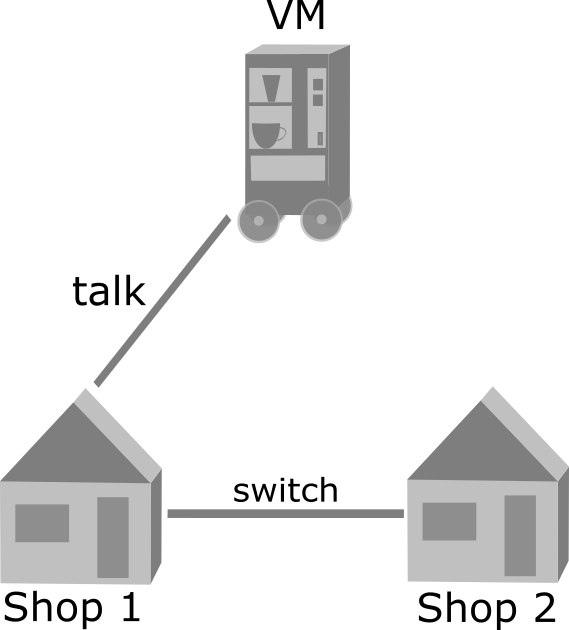
\includegraphics[width=0.45\textwidth]{./images/preliminaries/oz/oz_mobile_vending_machine_and_shops1.png}}}%
\hfill
\subcaptionbox{After switch}{\fbox{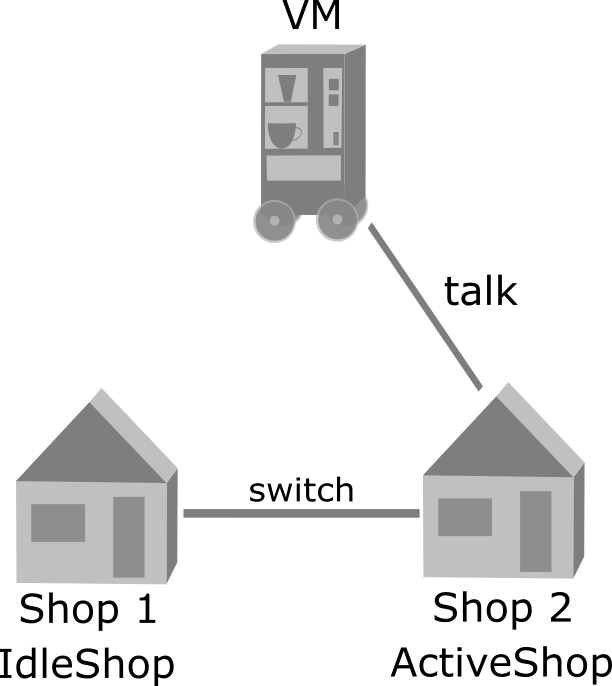
\includegraphics[width=0.45\textwidth]{./images/preliminaries/oz/oz_mobile_vending_machine_and_shops2.png}}}%
\caption{Mobile vending machine and shops}
\label{fig_oz_mobile_vending_machine_and_shops}%
\end{figure}

\begin{figure}[H]
\centering
\begin{sidebyside}
\begin{class}{ActiveShop(id: \integer)}
\\
\begin{state}
self, vmId, message: \integer
\\transferableOperation: nil | talk
\end{state} 
\\
\begin{init}
\\self = id
\\transferableOperation = talk
\end{init} 
\\
\begin{op}{switch\_\_\_\_\ then\ IdleShop}
x!: nil | talk
\ST
x! = transferableOperation
\\transferableOperation' = nil
\end{op}
\\
\begin{op}{talk}
\Delta (vmId, message)
\\y?, z?: \integer
\ST
y? = message'
\\z? = vmId'
\end{op}
\end{class}
\nextside
\begin{class}{IdleShop(id: \integer)}
\\
\begin{state}
self, vmId, message: \integer
\\transferableOperation: nil | talk
\end{state} 
\\
\begin{init}
\\self = id
\\transferableOperation = nil
\end{init} 
\\
\begin{op}{switch\_\_\_\_\ then\ ActiveShop}
\Delta (transferableOperation)
\\x?: nil | talk
\ST
x? = transferableOperation'
\end{op}
\end{class}
\end{sidebyside}
\caption{Active and idle shop.}
\label{fig_oz_active_idle_shop}
\end{figure}



\subsubsection{Restriction}
In this work when we use \oz{} to model an operation, we restrict our self to use only one type of parameters in the operation schema. Either input or output. This can be noticed in the operation schema $talk$ in:
\begin{itemize}
\item In \refFig{oz_vm_reference_name} all the parameters of the operation schema $talk$ are output paramaters.
\item In \refFig{fig_oz_unfixed_operation_schema_shop}  all the parameters of the operation schema $talk$ are input paramaters.
\end{itemize}
\textbf{Question:} why this restriction?\\
\textbf{Answer:} because a channel in \picalc{} is unidirectional pro reaction. In the next chapter we will map the \oz{} class constructs to  \picalc{} constructs, so we will map an \oz{} operation to an \picalc{} name , .i.e., channel. In \picalc{} a processes can send or receive over a channel pro reaction, but not the both together.